    \begin{figure}[!htbp]
        \centering
        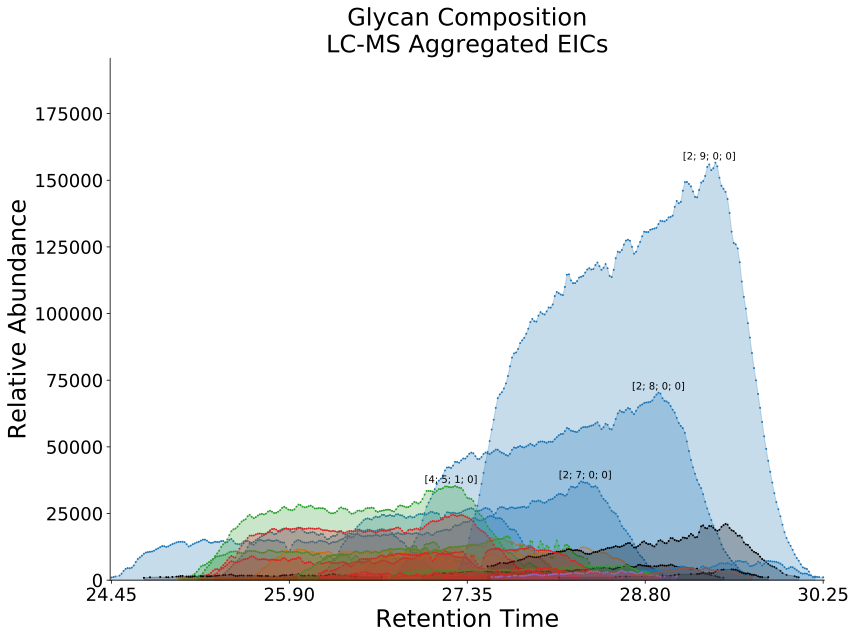
\includegraphics[width=0.45\textwidth,valign=t]{figure/phil_82_chromatograms.pdf}
        \includegraphics[width=0.45\textwidth,valign=t]{figure/phil_82_abundances.pdf}
        \caption{\textit{20141031-07-Phil-82} Glycan Relative Abundances}
        \label{fig:phil_82_aggregated_eics}
    \end{figure}

    \begin{table}
        \begin{minipage}[t]{0.25\linewidth}
            \vspace{0pt}
            (a)
            \centering
            
    \begin{tabular}{l | c}
        Group & $\tau$ \\
        \hline
        high-mannose & 15.88 \\
        hybrid & 12.12 \\
        bi-antennary & 0.00 \\
        asialo-bi-antennary & 18.57 \\
        tri-antennary & 0.00 \\
        asialo-tri-antennary & 11.61 \\
        tetra-antennary & 0.00 \\
        asialo-tetra-antennary & 6.18 \\
        penta-antennary & 0.00 \\
        asialo-penta-antennary & 0.00 \\
    \end{tabular}
    
            
        \end{minipage}
        \hspace{1cm}
        \begin{minipage}[t]{0.55\linewidth}
            \vspace{0pt}
            (b)
            \centering
            
    \begin{footnotesize}
    \begin{tabular}{l|p{2cm} p{2cm}}
Glycan Compostion &  Unregularized Score &  Regularized Score \\
\hline
\{Hex:5; HexNAc:2\}           &                14.89 &              15.23 \\
\{Hex:6; HexNAc:2\}           &                16.81 &              15.77 \\
\{Hex:7; HexNAc:2\}           &                17.27 &              16.33 \\
\{Hex:8; HexNAc:2\}           &                18.63 &              16.52 \\
\{Hex:9; HexNAc:2\}           &                19.10 &              16.20 \\
\{Hex:10; HexNAc:2\}          &                 6.80 &              13.94 \\
\{Hex:5; HexNAc:3\}           &                10.01 &              14.31 \\
\{Hex:6; HexNAc:3\}           &                17.03 &              15.17 \\
\{Fuc:1; Hex:6; HexNAc:3\}    &                16.76 &              15.20 \\
\{Hex:5; HexNAc:4\}           &                16.29 &              14.46 \\
\{Fuc:1; Hex:5; HexNAc:4\}    &                17.07 &              14.60 \\
\{Fuc:2; Hex:5; HexNAc:4\}    &                14.69 &              14.15 \\
\{Fuc:3; Hex:5; HexNAc:4\}    &                 7.75 &              13.12 \\
\{Hex:6; HexNAc:4\}           &                12.66 &              13.88 \\
\{Hex:5; HexNAc:5\}           &                16.43 &              13.35 \\
\{Fuc:1; Hex:5; HexNAc:5\}    &                16.51 &              13.36 \\
\{Hex:6; HexNAc:5\}           &                 6.74 &              11.68 \\
\{Fuc:1; Hex:6; HexNAc:5\}    &                10.94 &              12.15 \\
\{Fuc:2; Hex:6; HexNAc:5\}    &                 7.94 &              11.79 \\
\{Hex:7; HexNAc:6; Neu5Ac:4\} &                 6.39 &               1.06 \\
\{Fuc:1; Hex:7; HexNAc:6\}    &                 4.62 &               5.74 \\
\{Fuc:1; Hex:8; HexNAc:7\}    &                 8.16 &               3.49 \\
\end{tabular}

    \end{footnotesize}
    
        \end{minipage}
        \caption{
                 Search Results for \textit{20141031-07-Phil-82}.
                 (a) Estimated $\mathbf{\tau}$ for grid with ${\hat \gamma} = 15.372934$.
                 (b) Scores For Identified Glycans of grid with ${\hat \lambda} = 0.99$.}
        \label{tbl:phil_82_score_table}
    \end{table}
